\documentclass{prova}

\usepackage{amssymb}
\usepackage[inline]{enumitem}

\newcommand{\sen}{\,\mbox{sen}\,}
\newcommand{\tg}{\,\mbox{tg}\,}
\newcommand{\cosec}{\,\mbox{cosec}\,}
\newcommand{\cotg}{\,\mbox{cotg}\,}
\newcommand{\tr}{\,\mbox{tr}\,}
\newcommand{\ds}{\displaystyle}
\newcommand{\ra}{\rightarrow}

\professor{Prof.\@ Adriano Barbosa}
\disciplina{C\'alculo Diferencial e Integral}
\avaliacao{P2}
\curso{Eng.\@ de Energia}
\data{19/07/2018}

\begin{document}
	\cabecalho{5}  % o numero 5 indica a qnt de quadros na tabela de nota

	\textbf{Todas as respostas devem ser justificadas.}

	\begin{questionario}
        \q{Calcule o limite: $\ds\lim_{x\ra0^+} x \ln{x}$.}
        \q{Um tanque cil\'{\i}ndrico com raio de $10$ m enche com \'agua a uma
            taxa de $5$ m$^3$/min. Qu\~ao r\'apido a altura da \'agua est\'a aumentando?}
        \q{Um fazendeiro precisa cercar uma \'area retangular de $1000$ m$^2$ e
            em seguida dividir a \'area pela metade passando uma cerca paralela a um dos
            lados do terreno. Quais devem ser as dimens\~oes do terreno para que ele minimize
            o custo com a cerca?}
        \q{O gr\'afico de $g$ consiste em duas retas e um semic\'{\i}rculo. Use-o para
            calcular as integrais abaixo.}
            \begin{figure}[h]
                \centering
                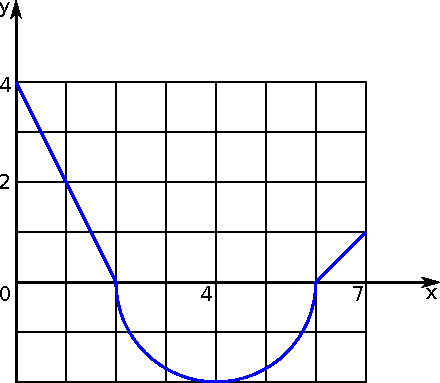
\includegraphics[width=0.4\textwidth]{q4.pdf}
            \end{figure}

            \begin{enumerate*}
                \item $\ds\int_6^7 g(x)\ dx$
                \hspace{0.5cm}
                \hspace{0.5cm}
                \item $\ds\int_4^6 g(x)\ dx$
                \hspace{0.5cm}
                \hspace{0.5cm}
                \item $\ds\int_4^7 g(x)\ dx$
            \end{enumerate*}
        \q{Calcule a integral $\ds\int_1^9 \frac{x-1}{\sqrt{x}}\ dx$.}
	\end{questionario}

\end{document}
